\section{Primitive di sincronizzazione}
La sincronizzazione è cruciale nei sistemi a memoria condivisa, ed è intrinsecamente indispensabile il supporto hardware per realizzare delle primitive di sincronizzazione. In particolare è necessaria un'istruzione atomica per leggere e poi scrivere la memoria. \uppercase{è} necessaria una nuova classe di istruzioni, ovvero le \textbf{atomic RMW} (read-modfiy-write).

\begin{lstlisting}[language={RISCAsm}]
* ATOMIC EXCHANGE 
* swap di un valore in memoria con un valore in un registro 
* se troviamo 0 nel registro il lock preso, 
* altrimenti continuiamo lo spinning

        EXCH    R5,0(R1)

* ESEMPIO DI SPINNING 
        MOVE    R2,#1 
LOOP    EXCH    R2,0(R1)
        BNE     LOOP 

* TEST AND SET 
* testa un valore in memoria, e se il valore nel registro 
* = 0, allora signicia che il lock e preso 

        TS      R3, 0(R1)

* FETCH AND INCREMENT 
* ritorna il valore di una locazione di memoria e  
* automaticamente lo incrementa 

        FI      R8,0(R1)

\end{lstlisting}

\noindent Le caches devono necessariamente essere progettate per supportare le istruzioni RMW, ad esempio per supportare un'operazione \textit{Read-Lock}, che recupera un blocco in stato E, invalida gli altri, e impedisce l'accesso al blocco agli altri finchè non viene rilasciato, e un'operazione \textit{Write-Unlock}, che fa un update e rilascia la linea. 

\begin{info}
    Quando si effettua lo spin su un lock, tericamente si perde tempo in busy wait. Questa cosa può essere evitata sfruttando l'evento di sincronizzazione globale di "sblocco" di una linea, quindi sfruttare un messaggio di gestione della coerenza per la sincronizzazione. Comunque le istruzioni atomiche generano un invalidazione, e di conseguenza un notevole traffico sul bus. Più semplicemente, possiamo iterare in lettura sulla variabile in cache e provare una costosa EXCH solo quando effettivamente il valore cambia. 
\end{info}

\begin{figure}[ht]
    \centering
    \setlength{\fboxrule}{0.5pt} % spessore sottile
    \setlength{\fboxsep}{0pt}    % senza spazio interno
    \fbox{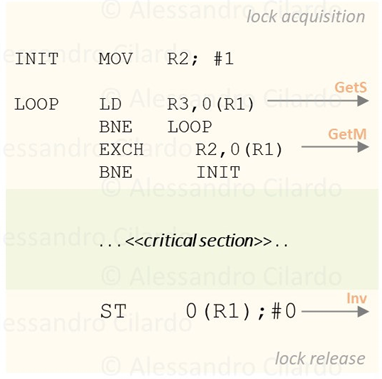
\includegraphics[width=0.4\textwidth]{fig/chapter_3/RWM.png}}
\end{figure}

\noindent Fare spin in lettura sulle caches locali riduce il traffico globale, ma sono necessari comunque messaggi di coerenza quando si rilascia e poi si acquisisce il lock. Se k core necessitano del lock, iniziano uno spin lock e ciò comporta che la variabile viene condivisa k volte. Il core che ottiene il lock acquisisce la variabile in stato M, e quando rilascia il lock sono inviati k-1 messaggi di invalidazione. Quindi la variabile viene ricopiata in memoria, e ricomincia il processo con K-1 cores. 
In definitiva si hanno $2k+1$ messaggi di gestione della coerenza per ogni occorrenza di acquisizione/rilascio del lock, e se N cores competono per il lock, allora il numero di messaggi globalmente sarà $2N+1 + 2(N-1)+1 + \dots + 2+1 = N^2 + N = O(N^2)$.

\noindent Le istruzioni RMW atomiche sono difficile da implementare, perchè richiedono due operazioni (di cui una di scrittura) in una sola ininterrompibile operazione. Ciò è difficile da realizzare in quanto la scrittura genera updates invalidanti per gli altri. La soluzione è aggiungere due particoalri istruzioni, denominate \textbf{Load Linked (LL)} (ritorna il valore iniziale della variabile lock, è un'operazione di lettura e non richiede traffico globale) e \textbf{Store Conditional} (ritorna 1 se ha successo, 0 altrimenti e non genera updates quando non ha successo). Queste istruzioni sono trasparenti in caso di fallimento di SC, e possono essere usate come base per altri meccanismi di sincronizzazione:

\begin{lstlisting}[language={RISCAsm}]
* ATOMIC EXCHANGE 
LOOP    MOVE    R3,R7 
        LL      R5,0(R1)
        SC      0(R1),R3 
        BNE     LOOP
        MOVE    R7,R5 

* FETCH AND INCREMENT 
LOOP    LL      R5,0(R1)
        ADD     R5,R5,#1
        SC      0(R1),R5 
        BNE     LOOP 
\end{lstlisting}
